% Basic LaTeX Template for Homework Submission with Formal Title Page
% Copyright (C) 2012 Patrick McLaren
% Copyright (C) April 2012 Joseph Paul Cohen (used style to create umb template)
%
%
% This program is free software: you can redistribute it and/or modify
% it under the terms of the GNU General Public License as published by
% the Free Software Foundation, either version 3 of the License, or
% (at your option) any later version.
%
% This program is distributed in the hope that it will be useful,
% but WITHOUT ANY WARRANTY; without even the implied warranty of
% MERCHANTABILITY or FITNESS FOR A PARTICULAR PURPOSE.  See the
% GNU General Public License for more details.
%
% You should have received a copy of the GNU General Public License
% along with this program.  If not, see <http://www.gnu.org/licenses/>.

\documentclass[12pt,letterpaper]{article}

\usepackage{amsmath,amsfonts,amsthm,amssymb}
\usepackage{setspace}
\usepackage{Tabbing}
\usepackage{lastpage}
\usepackage{extramarks}
\usepackage{chngpage}
\usepackage{soul,color}
\usepackage{graphicx,float,wrapfig}
\usepackage{tikz}
\usetikzlibrary{trees,snakes}
\usepackage[ruled,vlined,linesnumbered]{algorithm2e}
\usepackage{url}

%section ann subsectio have been changed so the indents look better
\makeatletter
%the following line was changed
\def\subsize{\@setsize\subsize{12pt}\xipt\@xipt}
\def\section{\@startsection{section}{1}{\z@}{24pt plus 2 pt
minus 2 pt} {12pt plus 2pt minus 2pt}{\large\bf}}
\def\subsection{\@startsection {subsection}{2}{\z@}{12pt
plus 2pt minus 2pt}{12pt plus 2pt minus 2pt}{\subsize\bf}}
\makeatother




% Author Info
\def\thetitle{Title}
\def\theauthor{Firstname Lastname}
\def\email{email@cs.umb.edu}
\def\theclass{CS999}
\def\studentid{Student ID\#}
\def\thedate{\today}
\def\university{University of Massachusetts Boston}

% Increase to 2.0 for double spacing.
\linespread{1}

% Header & Footers
% LaTeX has very generous margins, by default.
% I've shrunk the margins, considerably.
\usepackage[hmargin=2cm,vmargin=3.5cm]{geometry}
\usepackage{fancyhdr}
\pagestyle{fancy}
\lhead{\thetitle}
\chead{}
\rhead{\theauthor}
\lfoot{}
\cfoot{\theclass\ - \thedate}
\rfoot{\thepage}
\renewcommand{\headrulewidth}{0.5pt}
\renewcommand{\footrulewidth}{0.5pt}





\begin{document}

% Title Page
\begin{titlepage}
\begin{center}
\textsc{\LARGE \university}\vspace{10mm}
\hrule\vspace{2mm}
\huge\bfseries\thetitle\vspace{2mm}
\hrule\vspace{10mm}
\end{center}
\begin{flushleft}
\textbf\theauthor\\
\studentid\\
\email\\

\end{flushleft}
\vfill
\begin{center}
\thedate
\end{center}
\end{titlepage}

\newpage


\section*{Problem 1}

Why should you use this template?

\begin{enumerate}
  \item Latex makes it easier to have great looking homeworks
  \item Latex ``tex'' files work great with revision control systems such as
  $svn$ and $git$
  \item Math is much easier to write $\displaystyle\sum_{i=0}^\infty
  i(1-p^+)^{i-1}p^+ = \frac{p^+}{(1-(1-p^+))^2}$
\end{enumerate}


\section*{Problem 2}

You want to include images? Check out Figures \ref{fig:umblogo} and
\ref{fig:3umblogo}.

\begin{figure}[h]
\begin{center}

\includegraphics[width=.2\textwidth]{umass-boston-logo.png}
\caption{The UMASS Boston Logo}
\label{fig:umblogo}
\end{center}
\end{figure} 

\begin{figure}[h]
\begin{center}

\includegraphics[width=.2\textwidth]{umass-boston-logo.png}

\includegraphics[width=.2\textwidth]{umass-boston-logo.png}

\includegraphics[width=.2\textwidth]{umass-boston-logo.png}
\caption{The UMASS Boston Logo}
\label{fig:3umblogo}
\end{center}
\end{figure} 

\section*{Problem 3}

You want to draw a tree?  You can use the Tikz library.

\begin{figure}[h]
\center{
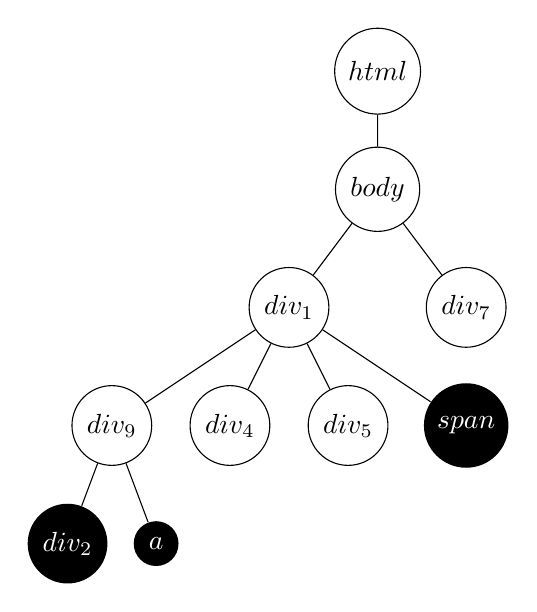
\begin{tikzpicture}[
level/.style={sibling distance=60mm/#1},
leaf/.style={circle, draw=none, fill=black,
        text centered, text=white}
]


\begin{scope}[xshift=+9cm, level/.style={sibling distance=45mm/#1}]
\node [circle,draw] (z){$html$}

% <body>
child {node [circle,draw] (body) {$body$}
% 	<div id="1">
	child {node [circle,draw] (1) {$div_1$}
% 		<div id="9">
		child {node [circle,draw] (9) {$div_9$}
% 			<div id="2">div2</div>
			child {node [circle,draw,leaf] (2) {$div_2$}}
% 			<a> a </a>
			child {node [circle,draw,leaf] (a) {$a$}}
		}
% 		</div>
% 		<div id="4"></div>
		child {node [circle,draw] (4) {$div_4$}	
	}
% 	</div>
% 		<div id="5">
		child {node [circle,draw] (5) {$div_5$}}
% 			<span id="6">span</span>
			child {node [circle,draw,leaf] (span) {$span$}}
		}
% 		</div>
% 	<div id="7"></div>
	child {node [circle,draw] (7) {$div_7$}}
};
% </body> 

\end{scope}
\end{tikzpicture}
}
\end{figure}


\section*{Problem 4}

You want to do some linear algebra?

$$V = \left(\begin{array}{c c c}
v_{1,1} & \ldots & v_{1,n}\\
\vdots & \ddots\\
v_{2,1} & \ldots & v_{2,n}\\
\vdots & \ddots\\
v_{m,1} & \ldots & v_{m,n}\\
\end{array}
\right)$$

$$\underbrace{rank(AB)}_n 
= \underbrace{rank(B)}_{\leq n}
-dim(\underbrace{null(A)}_0\cap \underbrace{range(B)}_n)$$

\begin{equation}
M_f = \left(\begin{array}{l l l}
a & b\\
c & d\\
\end{array}
\right) $$

$$M_f M_g = \left(\begin{array}{l l l}
ae+bg & af+bh\\
ce+dg & cf+dh\\
\end{array}
\right)
\end{equation}

\section*{Problem 5}

So you want to write an algorithm?

\begin{algorithm}[h]
\caption{\label{alg:sta}Simple Tree Matching}
\KwIn{Tree $a$ \\
\hspace{42pt}Tree $b$}
\KwOut{Integer $match$}

\If{a and b contain distinct symbols}{

return $0$

}\Else{

$m \leftarrow $ the number of first-level sub-trees of $a$

$n \leftarrow $ the number of first-level sub-trees of $b$

$M[i,0] \leftarrow 0 $ for $ i = 0,\ldots,m$

$M[0,j] \leftarrow 0 $ for $ j = 0,\ldots,n$

\For{$i = 1$ to $m$}{
	
	\For {$i = 1$ to $n$}{
		
		$x \leftarrow M[i,j-1]$
		
		$y \leftarrow M[i-1,j]$
		
		$z \leftarrow M[i-1,j-1]+ SimpleTreeMatch(a_i,b_j)$
		
		$M[i,j]	\leftarrow max(x,y,z)$
	}
}
return $M[m,n] + 1$
}

\end{algorithm}


\end{document}